\documentclass[12pt]{article}
\usepackage[utf8]{inputenc}

\usepackage{amsfonts}
\usepackage{amsmath}
\usepackage{bookmark}
\usepackage[a4paper, margin=3.5cm]{geometry}
\usepackage{graphicx} % For inserting images
\usepackage{hyperref} % For hyperlinks
\usepackage{indentfirst}
\usepackage{minted} % For code-highlighting
\usepackage{parskip}

\graphicspath{ {./images/} }
\setlength{\parindent}{15pt} % Set paragraph indentation
\setlength{\parskip}{1em} % Set paragraph space (one line)
\setminted{frame=single, breaklines} % Set codeblock style

\title{Programming Practicum Report:\\Final Test}
\author{\href{https://github.com/avaxar}{R. Ethan Halim}}
\date{November 25th, 2024}

\begin{document}

\maketitle

\section{P7: Find the Second Largest Number}
The entire source file is hosted on a GitHub repository \href{https://github.com/avaxar/uni-practica-1/tree/main/finals/01_second_max}{\textbf{here}}.

\subsection{Explanation}

In order to be able to find the second largest number within a given array without sorting, one must adapt the original algorithm to find the first largest number. However, in this adaptation, the loop keeps track of a second variable \texttt{secondMax} and within the handlers, they promote/demote the \texttt{firstMax} and \texttt{secondMax} variables accordingly. The pseudocode is as so.

\begin{minted}{text}
get numbers as an array of numbers

let firstMax be negative infinity
let secondMax be negative infinity

for each number in numbers
    if number > firstMax then
        secondMax = firstMax
        firstMax = number
    else if number > secondMax then
        secondMax = number

return secondMax
\end{minted}

The algorithm as a whole loops through the given array of its elements. Initially, \texttt{firstMax} and \texttt{secondMax} is set to the lowest possible value (ideally negative infinity). However, when the maximum encounters a number which is bigger than itself, it will promote the number to become the new maximum. The previous maximum is demoted as the second maximum. Additionally, if the number is lower than the maximum, but higher than the second maximum, it is promoted to become the second maximum. Implementation-wise, it is written as follows in C++:

\begin{minted}{cpp}
#include <bits/stdc++.h>

int64_t secondMax(const std::vector<int64_t>& numbers) {
    // Prerequisite variables: sets them as low as possible
    int64_t first = std::numeric_limits<int64_t>::min();
    int64_t second = first;

    // Loops through every number
    for (int64_t num : numbers) {
        // If exceeds the max, dethrones it
        if (num > first) {
            second = first; // Former max gets demoted.
            first = num;
        }
        // If exceeds the second max, dethrones it
        else if (num > second) {
            second = num;
        }
    }

    return second;
}
\end{minted}

In order to provide user input, in the \texttt{main} function, a simple CLI is implemented as follows, which requests for the array of numbers required by the function:

\begin{minted}{cpp}
int main() {
    // Requests for the amount of numbers
    size_t n;
    std::cout << "Enter the number of number(s): ";
    std::cin >> n;

    // Terminates early if no elements
    if (n == 0) {
        std::cout << "Expected to be more than zero.\n";
        return 1;
    }

    // Receives input for the numbers
    std::vector<int64_t> numbers(n);
    std::cout << "Input your numbers: ";
    for (size_t i = 0; i < n; i++) {
        std::cin >> numbers[i];
    }

    std::cout << "The second largest number is " << secondMax(numbers) << ".\n";
    return 0;
}
\end{minted}

% \pagebreak
\subsection{Manual Testing}
Below is the compilation and the testing of the source code.
\newline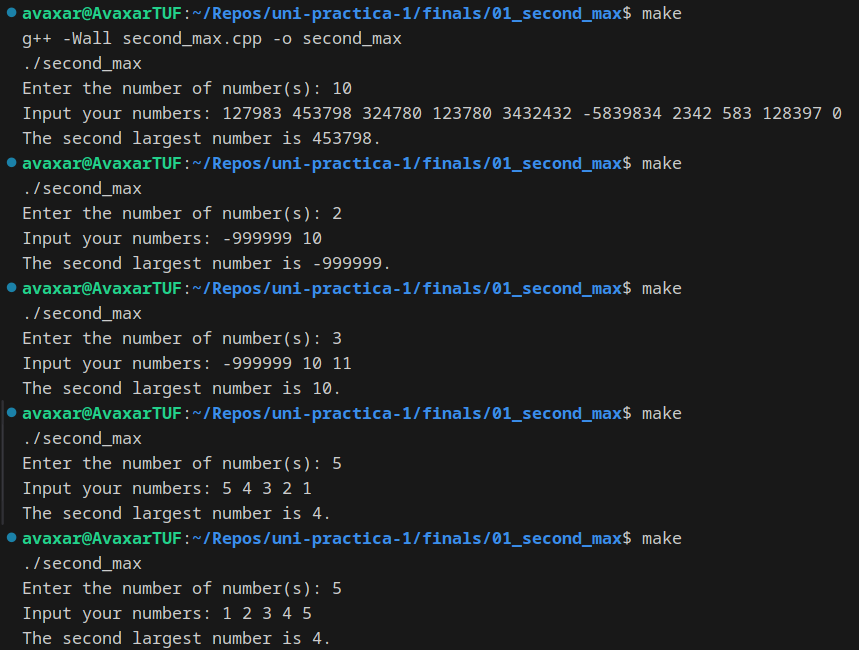
\includegraphics[width=\textwidth]{01_second_max}

% \pagebreak
\subsection{Test Cases}

\subsubsection{Tests}

Below is the hard-coded section of the program which tests for the program's output for a variety of cases. There exist 5 test cases.

\begin{minted}{cpp}
int main() {
    std::cout << "The program is running on testing mode...\n";
    int failures = 0;

    // Test #1
    if (secondMax({1, 2, 3, 4, 5}) != 4) {
        failures++;
        std::cout << "Test #1 failed!\n";
    }

    // Test #2
    if (secondMax({8234, 324, 323, 1239, 4523, 1392}) != 4523) {
        failures++;
        std::cout << "Test #2 failed!\n";
    }

    // Test #3
    if (secondMax({-999999, 3129, 54240, 123}) != 3129) {
        failures++;
        std::cout << "Test #3 failed!\n";
    }

    // Test #4
    if (secondMax({0, -1, -2, -3, -4, -5, -6, -7, -8, -999}) != -1) {
        failures++;
        std::cout << "Test #4 failed!\n";
    }

    // Test #5
    if (secondMax({-2, -3, -4, -1, 0, 1}) != 0) {
        failures++;
        std::cout << "Test #5 failed!\n";
    }

    if (failures > 0) {
        std::cout << failures << " test(s) failed.\n";
        return 1;
    }
    else {
        std::cout << "The test case(s) ran successfully\n.";
        return 0;
    }
}
\end{minted}

\subsubsection{Execution}
Below are the results of the test cases. No test cases failed.
\newline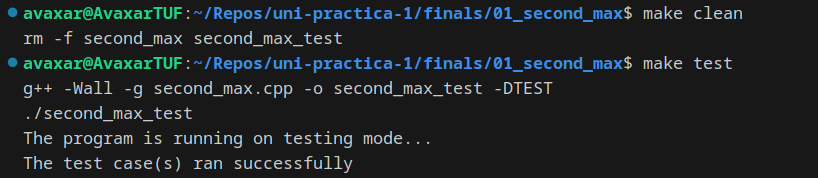
\includegraphics[width=\textwidth]{01_second_max_test}

\section{P3: Count Odd and Even Numbers}
The entire source file is hosted on a GitHub repository \href{https://github.com/avaxar/uni-practica-1/tree/main/finals/02_count_odd_even}{\textbf{here}}.

\subsection{Explanation}

In order to count the number of odd and even numbers in a given array, one can iterate through the elements of the said array and check for both cases. In the pseudocode below, there exists counter variables \texttt{odds} and \texttt{evens}, which represent the number of the two types of numbers. For every number, if it's even, the program increments \texttt{evens}; if it's odd, the program increments \texttt{odds}.

\begin{minted}{text}
get numbers as an array of numbers

let odds be an integer, 0
let evens be an integer, 0

for each number in numbers
    if number is even then
        evens = evens + 1
    if number is odd then
        odds = odds + 1

return odds, evens
\end{minted}

The pseudo-expressions \texttt{is even} and \texttt{is odd} can be implemented realistically using the modulo operator by checking the remainder of the number by two.
$$x \text{ is even} \equiv x \text{ mod } 2 = 0$$
$$x \text{ is odd} \equiv \neg(x \text{ is even})$$

It is implemented as below in C++. Note that since returning multiple return values is not possible in C++ without a structure, an array, or \texttt{std::tuple}, the function returns the \texttt{odds} and \texttt{evens} variables through reference parameters.

\begin{minted}{cpp}
#include <bits/stdc++.h>

void count(const std::vector<int64_t>& numbers, size_t& odds, size_t& evens) {
    odds = 0;
    evens = 0;

    // Loops through every number
    for (int64_t num : numbers) {
        // If even
        if (num % 2 == 0) {
            evens++;
        }
        // If odd
        else {
            odds++;
        }
    }
}
\end{minted}

In order to provide user input, in the \texttt{main} function, a simple CLI is implemented as follows, which requests for the array of numbers required by the function:

\begin{minted}{cpp}
int main() {
    // Requests for the amount of numbers
    size_t n;
    std::cout << "Enter the number of number(s): ";
    std::cin >> n;

    // Terminates early if no elements
    if (n == 0) {
        std::cout << "Expected to be more than zero.\n";
        return 1;
    }

    // Receives input for the numbers
    std::vector<int64_t> numbers(n);
    std::cout << "Input your numbers: ";
    for (size_t i = 0; i < n; i++) {
        std::cin >> numbers[i];
    }

    // Counts the amount of odd and even numbers
    size_t odds, evens;
    count(numbers, odds, evens);


    std::cout << "There are " << odds << " odd number(s) and " << evens << " even number(s).\n";
    return 0;
}
\end{minted}

% \pagebreak
\subsection{Manual Testing}
Below is the compilation and the testing of the source code.
\newline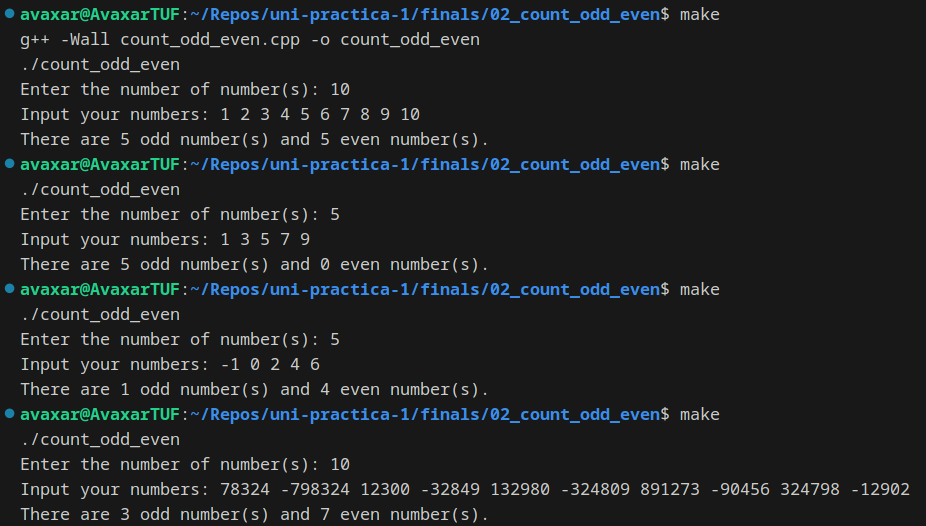
\includegraphics[width=\textwidth]{02_count_odd_even}

% \pagebreak
\subsection{Test Cases}

\subsubsection{Tests}

Below is the hard-coded section of the program which tests for the program's output for a variety of cases. There exist 5 test cases.

\begin{minted}{cpp}
int main() {
    std::cout << "The program is running on testing mode...\n";
    int failures = 0;

    size_t odds, evens;

    // Test #1
    count({1, 2, 3, 4, 5, 6, 7, 8, 9, 10}, odds, evens);
    if (odds != 5 || evens != 5) {
        failures++;
        std::cout << "Test #1 failed!\n";
    }

    // Test #2
    count({13289, 123987, 98234, 32478, 123789, 54312, 213980, 4503, 341980, 42978}, odds, evens);
    if (odds != 4 || evens != 6) {
        failures++;
        std::cout << "Test #2 failed!\n";
    }

    // Test #3
    count({0, 2, 4, 6, 10, 12, 14, 16, 18, 20}, odds, evens);
    if (odds != 0 || evens != 10) {
        failures++;
        std::cout << "Test #3 failed!\n";
    }

    // Test #4
    count({-1, 1, 3, 5, 7, 9, 11, 13, 15, 17}, odds, evens);
    if (odds != 10 || evens != 0) {
        failures++;
        std::cout << "Test #4 failed!\n";
    }

    // Test #5
    count({0, 1, -2, 3, -4, 5, -6, 7, -8, 9}, odds, evens);
    if (odds != 5 || evens != 5) {
        failures++;
        std::cout << "Test #5 failed!\n";
    }

    if (failures > 0) {
        std::cout << failures << " test(s) failed.\n";
        return 1;
    }
    else {
        std::cout << "The test case(s) ran successfully\n.";
        return 0;
    }
}
\end{minted}

\subsubsection{Execution}
Below are the results of the test cases. No test cases failed.
\newline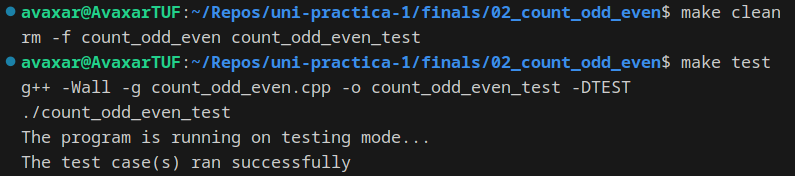
\includegraphics[width=\textwidth]{02_count_odd_even_test}

\end{document}
